% ============================================================
%  SCHOLA DOMESTICA — Level 1, Week 1, Lesson 3
%  Topic: Numbers 4 and 5
% ============================================================
\documentclass[12pt,letterpaper]{article}
\usepackage[top=1in,bottom=1in,left=1in,right=1in]{geometry}
\usepackage{fontspec}\usepackage{graphicx}\usepackage{xcolor}
\usepackage{mdframed}\usepackage{tikz}\usepackage{fancyhdr}\usepackage{parskip}
\usetikzlibrary{shapes.geometric}
\setmainfont{EB Garamond}[Ligatures=TeX,Numbers=OldStyle]
\definecolor{sd-blue}{RGB}{60,100,160}\definecolor{sd-gold}{RGB}{180,140,50}
\definecolor{sd-light}{RGB}{245,242,235}\definecolor{sd-green}{RGB}{70,130,80}
\pagestyle{fancy}\fancyhf{}
\fancyhead[L]{\small\color{sd-blue}\textit{Schola Domestica Mathematics}}
\fancyhead[R]{\small\color{sd-blue}\textit{Level~1 \(\cdot\) Week~1 \(\cdot\) Lesson~3}}
\fancyfoot[C]{\small\color{sd-blue}1}
\renewcommand{\headrulewidth}{0.4pt}
\newmdenv[backgroundcolor=sd-light,linecolor=sd-blue,linewidth=1pt,
  innerleftmargin=10pt,innerrightmargin=10pt,innertopmargin=8pt,
  innerbottommargin=8pt,roundcorner=4pt]{instructbox}
\newmdenv[backgroundcolor=white,linecolor=sd-green,linewidth=1.5pt,
  innerleftmargin=10pt,innerrightmargin=10pt,innertopmargin=8pt,
  innerbottommargin=8pt,roundcorner=4pt]{checkbox}
\newcommand{\ansblank}{\underline{\hspace{1.6cm}}}
\newcounter{probnum}
\newcommand{\prob}{\stepcounter{probnum}\noindent\textbf{\arabic{probnum}.}\quad}
\newcommand{\onestar}{
\begin{tikzpicture}[baseline=-0.1cm]
  \node[star,star points=5,star point ratio=2.5,fill=sd-gold,
        draw=sd-gold!80!black,minimum size=0.9cm]{};
  \end{tikzpicture}}
\newcommand{\onedot}{
\begin{tikzpicture}[baseline=-0.05cm]
  \fill[sd-blue](0,0)circle(0.22cm);
  \end{tikzpicture}}
\begin{document}
\begin{center}
  {\color{sd-blue}\Large\bfseries Schola Domestica Mathematics — Level~1}\\[4pt]
  {\color{sd-blue}\rule{\linewidth}{1.5pt}}\\[6pt]
  {\LARGE\bfseries Lesson 3 \quad|\quad Numbers 4 and 5}\\[4pt]
  {\color{sd-gold}\rule{\linewidth}{0.8pt}}
\end{center}
\vspace{4pt}
\begin{instructbox}
\noindent\textbf{\color{sd-blue}Instruction:}\\[4pt]
Today we meet \textbf{4} and \textbf{5}.
Hold up four fingers, then add one more — that is five.
Five fingers fill one whole hand!
\end{instructbox}
\vspace{8pt}
\noindent\textbf{\color{sd-blue}Trace and write:}
\vspace{4pt}
\begin{center}
\begin{tabular}{|c|c|c|c|c|c|c|c|}
\hline
\rule{0pt}{26pt}{\Huge\color{sd-blue!40}4}&{\Huge\phantom{4}}&{\Huge\phantom{4}}&{\Huge\phantom{4}}&
{\Huge\color{sd-blue!40}5}&{\Huge\phantom{5}}&{\Huge\phantom{5}}&{\Huge\phantom{5}}\\
\hline
\end{tabular}
\end{center}
\vspace{4pt}{\color{sd-gold}\rule{\linewidth}{0.5pt}}\vspace{4pt}
\noindent\textbf{\color{sd-blue}Practice}\vspace{4pt}

\prob Count the dots.\quad\onedot\onedot\onedot\onedot\quad\ansblank

\vspace{8pt}
\prob Count the dots.\quad\onedot\onedot\onedot\onedot\onedot\quad\ansblank

\vspace{8pt}
\prob How many? \quad
\IfFileExists{stars_5.jpg}{
\includegraphics[height=1.4cm]{stars_5.jpg}}{%
  \onestar\onestar\onestar\onestar\onestar}
\quad\ansblank

\vspace{8pt}
\prob How many? \quad
\IfFileExists{apples_4.jpg}{
\includegraphics[height=1.4cm]{apples_4.jpg}}{%
  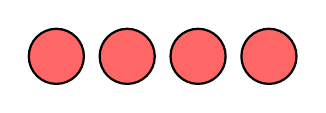
\begin{tikzpicture}[baseline=0]
    \foreach \x in {0,1,2,3}\draw[fill=red!60,thick](\x*0.9,0)circle(0.35);
  \end{tikzpicture}}
\quad\ansblank

\vspace{8pt}
\prob Circle the correct number for this group: \quad
  \IfFileExists{ducks_4.jpg}{
\includegraphics[height=1.4cm]{ducks_4.jpg}}{%
    
\begin{tikzpicture}[baseline=0]
      \foreach \x in {0,1,2,3}\draw[fill=yellow!70,thick](\x*0.9,0)ellipse(0.35 and 0.25);
    \end{tikzpicture}}
  \quad{\Large 3 \quad \textbf{4} \quad 5}

\vspace{8pt}
\prob Draw \textbf{4} flowers in the box:
\vspace{2pt}
\noindent\fbox{\rule{0pt}{2cm}\hspace{9cm}}

\vspace{8pt}
\prob \textit{(Teacher reads)} A bird had 3 eggs in her nest.
She laid 2 more eggs. Now how many eggs are there? \quad\ansblank
\textit{(Hint: count all the eggs.)}

\vspace{8pt}
\prob Write the numbers 1 through 5 in order:\\[4pt]
\hspace{1cm}\ansblank\quad\ansblank\quad\ansblank\quad\ansblank\quad\ansblank

\vspace{8pt}
\prob What number comes right after 4? \quad\ansblank

\vspace{6pt}
\prob What number comes right before 5? \quad\ansblank

\vspace{6pt}{\color{sd-gold}\rule{\linewidth}{0.5pt}}\vspace{4pt}
\begin{checkbox}
\noindent\textbf{\color{sd-green}Knowledge Check}\\[4pt]
\setcounter{probnum}{0}
\prob \IfFileExists{stars_4.jpg}{
\includegraphics[height=1.2cm]{stars_4.jpg}}{%
  \onestar\onestar\onestar\onestar}\quad\ansblank\\[8pt]
\prob How many fingers on one hand? \quad\ansblank
\end{checkbox}
\vfill
\noindent{\color{sd-blue}$\bigstar$ \textbf{Enrichment:}}
In Latin: \textit{ūnus, duo, tr\={e}s, quattuor, quīnque}.
Can you say all five?
\vspace{4pt}\hrule\vspace{2pt}
{\footnotesize\color{gray}\textit{Teacher note: Five is a critical anchor number. Spend extra time if needed.}}
\end{document}
